\begin{figure}[h]
  \centering
  \begin{tabular}{ p{4cm} p{5cm} p{5cm} }
    \centering 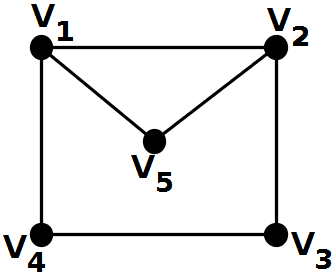
\includegraphics[width=3cm]{./img/envelope.png} & 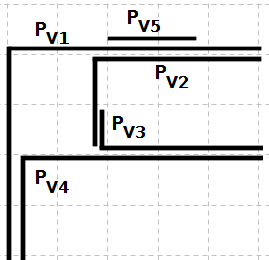
\includegraphics[width=4cm]{./img/envelopeHellyGradeTransparente.png} & 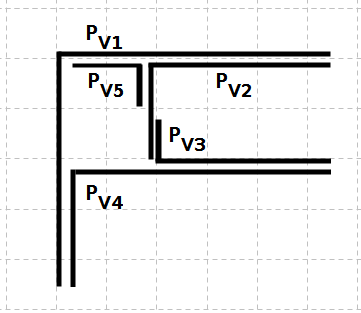
\includegraphics[width=4.6cm]{./img/envelopeNaoHellyGrade.png}
    \\
    \footnotesize \centering (a) Um grafo com  5 vértices & \footnotesize(b) Uma representação $B_1$-EPG que satisfaz a propriedade Helly & \footnotesize (c) Uma representação $B_1$-EPG que não satisfaz a propriedade Helly  \\

  \end{tabular}
\caption{Um grafo com 5 vértices em (a) e algumas representações de dobra simples: uma representação Helly em (b) e outra representação que não satisfaz a propriedade Helly em (c)} \label{fig:envelopeRepresentacoes}
\end{figure}